\section{Introduction}
\label{sec:intro}

Abstraction is the key to managing software complexity.
%
Experienced programmers routinely extract common functionality
into libraries of reusable abstractions
to express their intent more clearly and concisely.
%
What if this process of extracting useful abstractions from code could be automated?
%
\emph{Library learning} seeks to answer this question
  with techniques to compress
  a given corpus of programs
  by extracting common structure into reusable library functions.
%
Library learning
  has many potential applications
  from refactoring and decompilation~\cite{szalinski,shapemod},
  to modeling human cognition~\cite{cogsci-smiley,cogsci-dataset},
  and speeding up program synthesis by
  specializing the target language to
  a chosen problem domain~\cite{dreamcoder}.

Consider the simple library learning task in \autoref{fig:polygons}.
On the left,
 \autoref{fig:polygons}a shows a corpus of three programs in a
 \cogsci DSL from \citet{cogsci-dataset}.
Each program corresponds to a picture
 composed of regular polygons,
 each of which is made of multiple rotated line segments.
On the right,
 \autoref{fig:polygons}b shows a learned library
 with a single function (named \T{f0})
 that abstracts away the construction of scaled regular polygons.
The three input programs can then be refactored
 into a more concise form using the learned \T{f0}.
% In this case,
%  abstracting regular polygons is intuitively ``correct'',
%  but in general, this is a qualitative choice.
Whether \T{f0} is the ``best'' abstraction for this corpus is generally hard to quantify.
%
For this paper,
 we follow \dc~\cite{dreamcoder} and use \emph{compression} as a
 metric for library learning, \ie,
 the goal is to reduce the total size of the corpus in AST nodes
 (from 208 to 72 \autoref{fig:polygons}).
%
Importantly, the total size of the corpus includes the size of the library:
this prevents library learning from generating too many overly-specific functions,
and instead biases it towards more general and reusable abstractions. % that can be reused multiple times.

\begin{figure}
    \centering
    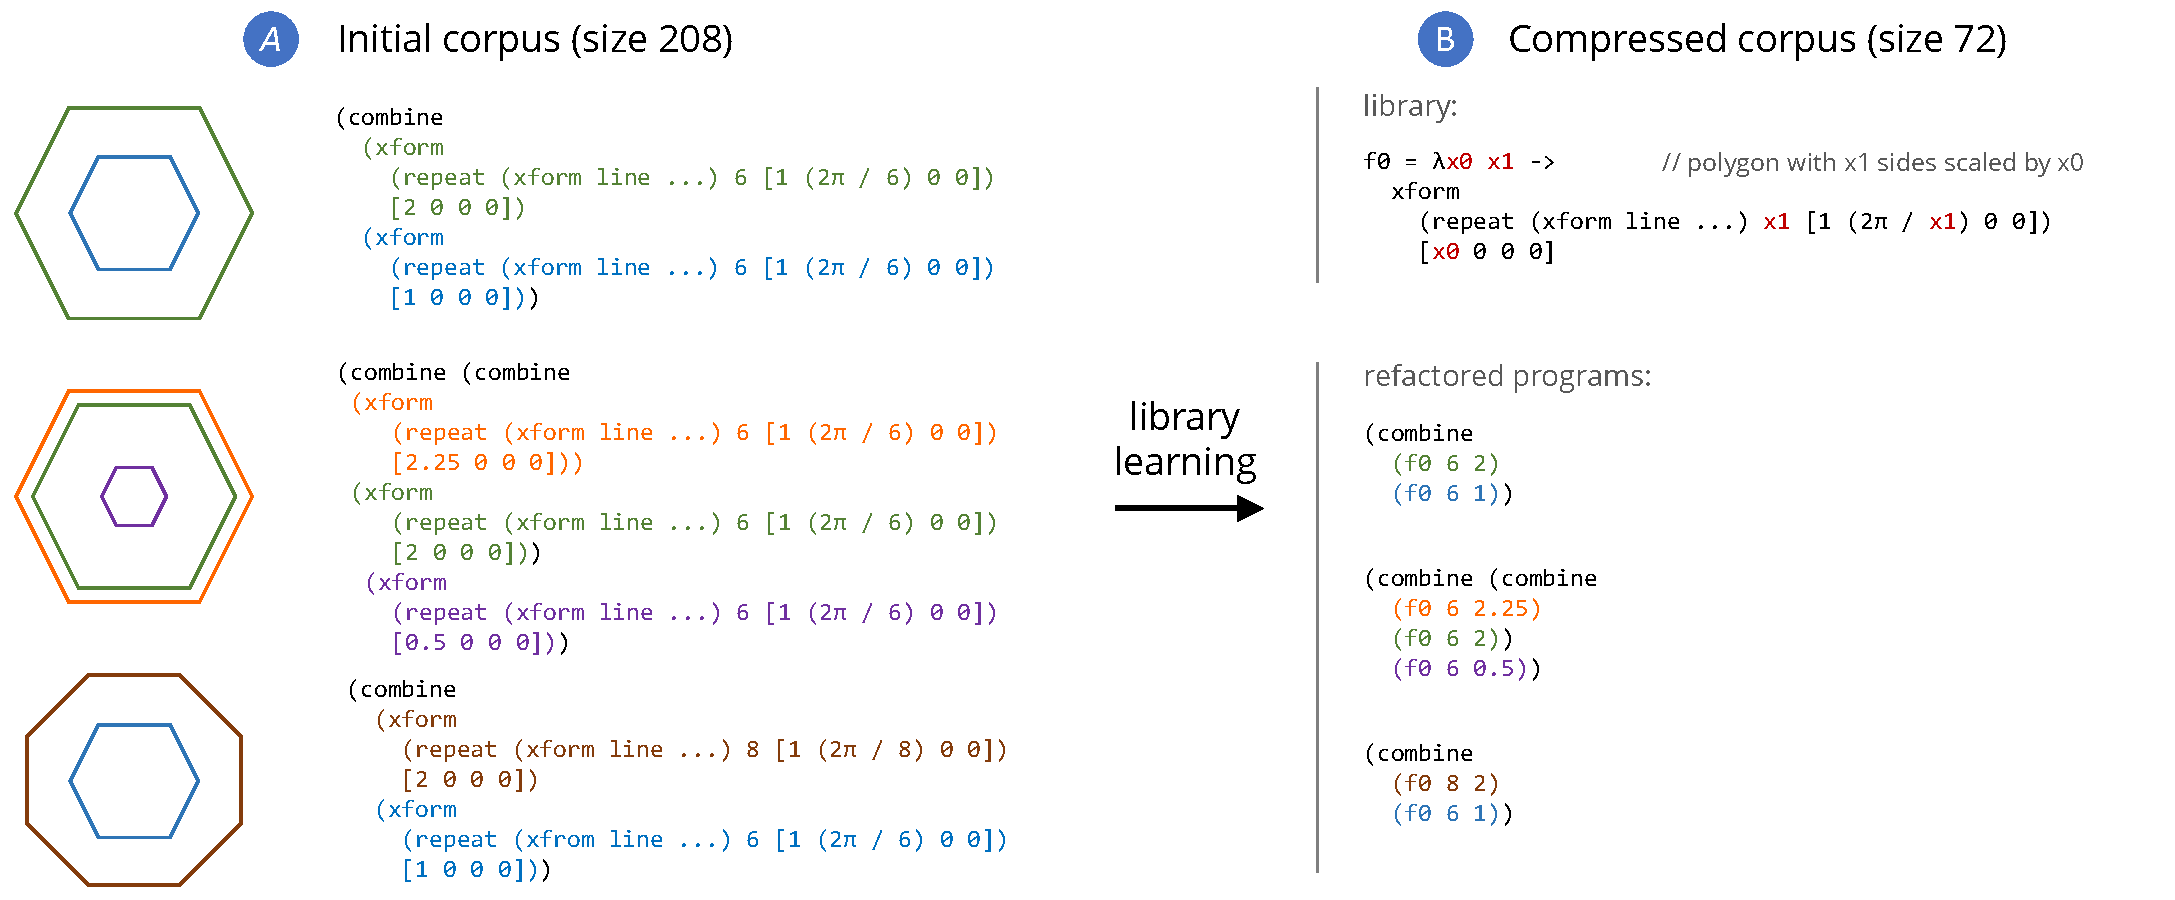
\includegraphics[width=\textwidth]{figures/polygons.pdf}
    \caption{Example of library learning.
             Initial corpus A contains three graphical programs from the ``nuts \& bolts'' dataset of \citet{cogsci-dataset}.
             Corpus B is the output of library learning with a single learned function for a scaled polygon,
             and the original programs refactored using this function.}\label{fig:polygons}
\end{figure}

Library learning can be phrased as a program synthesis problem
 structured in two phases:
%  \textit{Generate} -- generating candidate abstractions, and then
%  \textit{Select} -- selecting those abstractions that produce the best (smallest)
\emph{generating} candidate abstractions, and then
\emph{selecting} those abstractions that produce the best (smallest)
     refactored corpus.
The state-of-the-art technique, implemented in \dc~\cite{dreamcoder},
  suffers from two primary limitations % in the \textit{Generate} phase
  that hinder scaling library learning to larger and more realistic inputs.
\begin{itemize}
    \item
    Candidate generation is not \emphbf{precise}:
    \dc generates many candidate abstractions that cannot be useful,
    slowing down the selection phase and the algorithm as a whole.
    % The result is that many candidates are sent to the selection phase
    %  that should never be selected, slowing down the algorithm as a whole.
    \item
    % Candidate generation is not \emphbf{robust} to syntactic variation.
    % Candidate generation is not \emphbf{robust}:
    The technique is purely syntactic and hence not \emphbf{robust} to superficial variation.
    % \dc proposes library function candidates purely syntactically
    % and hence is brittle to superficial variation.
    For example,
     a human programmer would immediately know that the terms $2 + 1$ and $1 + 3$
     can be refactored using the abstraction $\lambda x \bnd x + 1$,
     because addition commutes;
     a purely syntactic library learning approach cannot generate this abstraction.
    % For example,
    %  a purely syntactic algorithm cannot
    %  generate an abstraction for the programs $2 + 1$ and $1 + 3$.
    % However,
    %  since we know that addition commutes,
    %  $\lambda x \bnd x + 1$ applies in both programs.
    % \item
    % \mw{something about beam extraction}
\end{itemize}
In this paper we propose \emph{library learning modulo (equational) theories} (LLMT)---%
a new library learning algorithm
that addresses both of the above limitations.
% from the \textit{Generate} phase of library learning.

\mypara{Precise Candidate Generation via Anti-Unification}
%
To make candidate generation more precise,
%To make the proposal stage of library learning more precise,
 LLMT leverages two key observations:
\begin{itemize}
    \item
    Useful abstractions must be used in the corpus at least twice.
    %
    For example, in a corpus of two programs $2 + 1$ and $3 + 1$,
    there is no need to consider $\lambda x \bnd 3 + x$
    because it can only be used in one place,
    and hence would only increase the size of the corpus.
    %% Nadia: there's nothing wrong with using this example,
    %% but the asymmetry with the second example annoys me.
    % For example, there is no need to consider $\lambda x \bnd \T{trans}\ x\ [0.5\ 0\ 0\ 0]$
    %  in our running example,
    %  because it can only be used in one place;
    %  it would only increase the size of the program.
    \item
    Abstractions should be ``as concrete as possible'' for a given corpus.
    For example,
     in the same corpus with $2 + 1$ and $3 + 1$,
     the abstraction $\lambda x \bnd x + 1$
     is superior to the more general
     $\lambda x\ y \bnd x + y$,
     since both apply to the same two terms,
     but applying the latter is more expensive (it requires two arguments).
    %  since the argument for $y$ in the latter would always be $1$.
    % In our example, the chosen \texttt{f0} of
    %   $\lambda x \bnd \T{repeat}\ (\T{trans line}\ \ldots)\ x\ [1\ (2\pi / x)\ 0\ 0]$
    %   is superior
    %   the more general
    %   $\lambda x\ y \bnd \T{repeat}\ (\T{trans line}\ \ldots)\ x\ y$,
    %   because the argument for $y$ in the latter abstraction will always be exactly
    %   $[1\ (2\pi / x)\ 0\ 0]$.
\end{itemize}
%
In other words, a useful abstraction corresponds to the least general \emph{pattern}
that matches some pair of subterms from the original corpus;
such a pattern can be computed via \emph{anti-unification} (AU)~\cite{plotkin1970lattice}.
%
For example, anti-unifying $2 + 1$ and $3 + 1$
  yields the pattern $X + 1$,
  and the desired candidate library function $\lambda x \bnd x + 1$
  can be derived by abstracting over the pattern variable $X$.
  % \footnote{Hereafter, we use upper-case letters for pattern variables and lower-case letters for program variables.}
%
Similarly, in \autoref{fig:polygons}, the abstraction \T{f0} can be derived
 by anti-unifying, for example, the blue and the brown subterms of the corpus.
%
% The remaining challenge is to efficiently compute the set of anti-unifiers
% between \emph{all} pairs of subterms in the corpus;
% LLMT achieves this via a new bottom-up dynamic programming algorithm.

\mypara{Robustness via E-Graphs}
%
To make candidate generation more robust,
%To address the robustness issue,
LLMT additionally takes as input a \emph{domain-specific equational theory} % (expressed as a set of rewrite rules)
and uses it to find programs that are semantically equivalent to the original corpus,
but share the most syntactic structure.
%
For example, in the domain of arithmetic, we expect the theory to contain the equation
$X + Y  \semeq  Y + X$,
which states that addition is commutative.
%
Given the corpus with terms $2 + 1$ and $1 + 3$,
this rule can be used to rewrite the second term in to $3 + 1$,
enabling the discovery of the common abstraction $\lambda x \bnd x + 1$.

% For example, for the graphical DSL from our running example,
% the equational theory might contain a rule that adds a unit transformation to any shape $s$:
% $$
% s  \Rightarrow  \T{trans}\ s\ [1\ 0\ 0\ 0]
% $$
% %
% This rule can then be used to transform the two unit hexagons in corpus C from \autoref{fig:llmt}
% into the form they have in the original corpus in \autoref{fig:polygons},
% which enabled the discovery of the scaled polygon abstraction $f_0$
% and using it to compress the corpus to size 72.

The main challenge with this approach is to search over the large space of programs
that are semantically equivalent to the original corpus.
%
To this end, LLMT relies on the \emph{e-graph} data structure
and the \emph{equality saturation} technique~\cite{tate2009equality,willsey2021egg}
to compute and represent the space of semantically equivalent programs.
%
To enable efficient library learning over this space,
% we extend our AU-based candidate generation algorithm to work over e-graphs.
we propose a new candidate generation algorithm
that efficiently computes the set of all anti-unifiers
between pairs of sub-terms represented by an e-graph,
using dynamic programming.

Finally, \emph{selecting} the optimal library
%   (the \textit{Select} phase of library learning)
  in this setting reduces to the problem of
  \emph{extracting} the smallest term out of an e-graph
  in the presence of common sub-expressions.
%
This problem is extremely computationally intensive in its general form,
and existing approaches have limited scalability~\cite{tensat}.
%
Instead we propose \emph{targeted subexpression elimination}:
a novel e-graph extraction algorithm
that uses domain-specific knowledge to reduce the search space
and readily supports approximation via beam search to trade off accuracy and efficiency.
% Finally, to select the optimal library,
% we propose \emph{beam extraction}:
% a new algorithm for extracting the best term from an e-graph,
% which is based on beam search and can trade off accuracy and efficiency.

\begin{figure}
    \centering
    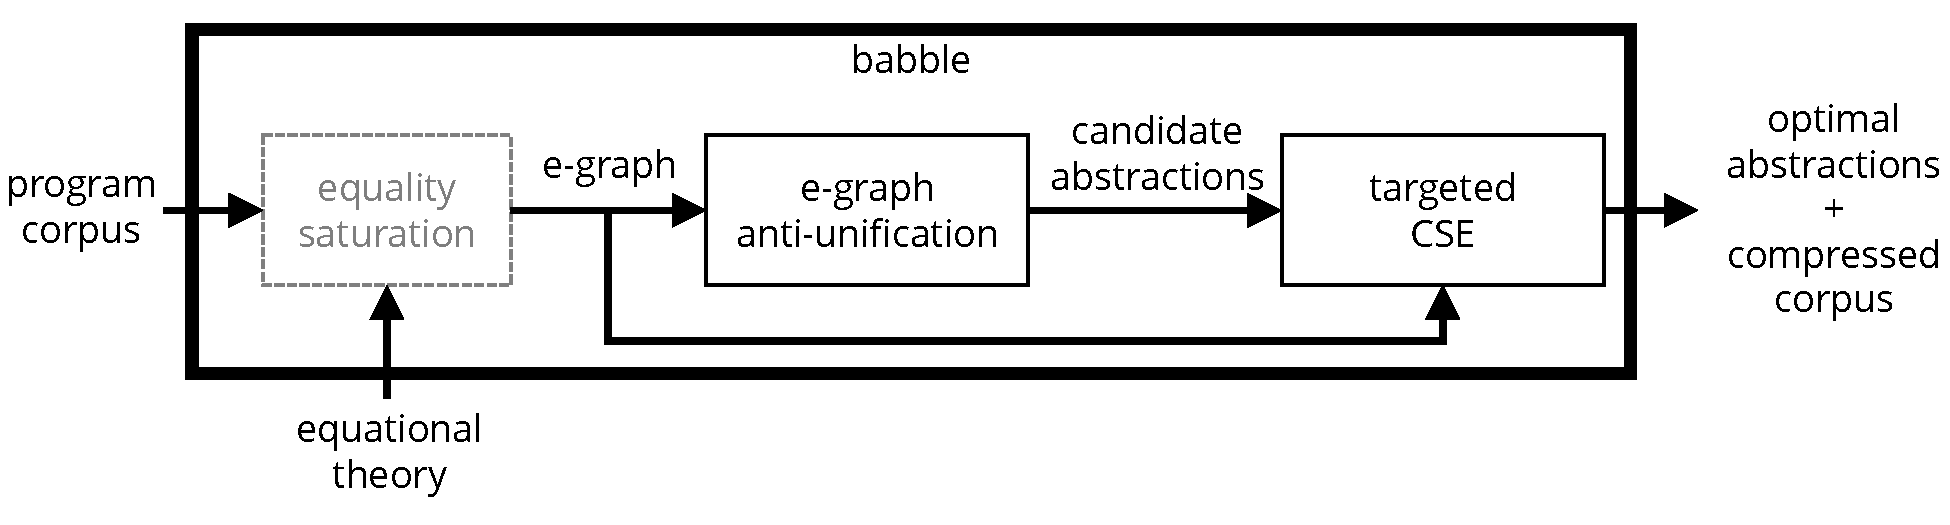
\includegraphics[width=.8\textwidth]{figures/arch.pdf}
    \caption{\tool architecture overview}\label{fig:arch}
  \end{figure}


\mypara{\tool}
%
We have implemented LLMT in \tool,
a tool built on top of the \tname{egg} e-graph library~\cite{willsey2021egg}.
%
The overview of the \tool's workflow is shown in \autoref{fig:arch},
with gray boxes representing existing techniques
and black boxes representing our contributions.
% Given the input corpus and rewrite rules from \autoref{fig:llmt},
% \tool is able to discover the abstraction $f_0$ and the compressed corpus B
% in a fraction of a second.

We evaluated \tool on benchmarks from two sources:
compression tasks extracted from \dc runs~\cite{compression-bench}
and \cogsci programs used to evaluate concept learning in humans~\cite{cogsci-dataset}.
%
Our evaluation shows that \tool outperforms \dc on its own benchmarks,
 achieving better compression in orders of magnitude less time.
Adding domain-specific rewrites improves compression even further.
%
We also show that \tool scales to the larger \cogsci corpora,
which is beyond reach of \dc.
% %
% Although adding domain-specific rewrites does impact scalability,
% it also makes the results more robust to syntactic variations in the corpus.
%
We also present and discuss a selection of abstractions learned by \tool,
 demonstrating that the LLMT approach can learn functions that match human intuition.


\mypara{Contributions}
%
In summary, this paper makes the following contributions:
%
\begin{itemize}
    \item \emph{library learning modulo equational theory}:
        a library learning algorithm that can incorporate an arbitrary domain-specific equational theory
        to make learning robust to syntactic variations;
    \item \emph{e-graph anti-unification}:
        an algorithm that efficiently generates the set of candidate abstractions
        using the mechanism of anti-unification extended from terms to e-graphs;
%   \item an anti-unification algorithm that operates on e-graphs rather than
%         concrete terms,
  \item \emph{targeted common subexpression elimination}:
        a new approximate algorithm for extracting the best term from an e-graph
        in the presence of common sub-expressions.
\end{itemize}



%%%%%%%%%%%%%%%%%%
% OLD TEXT BELOW %
%%%%%%%%%%%%%%%%%%
\begin{comment}

In this work, we consider the problem of library learning
as formulated in \dc~\cite{dreamcoder}.
%
At a high level, the goal of library learning is to \emph{compress} a given corpus of programs
by inventing a library of abstractions and refactoring the corpus using this library.
%
\autoref{fig:polygons} shows a simple instance of library learning
over three graphical programs sampled from the dataset of \citet{cogsci-dataset}.
%
The original programs are expressed in a vector graphics DSL
with constructs for primitive shapes (\eg \T{line}),
applying a transformation matrix to a shape (\T{trans}),
and repeating a shape $n$ times, with a transformation applied between iterations (\T{repeat}).
%
Although this is not immediately obvious from the programs themselves,
looking at the corresponding images makes it clear that
each program describes several nested polygons (hexagons and octagons) at different scales.
%
If we abstract the concept of a scaled polygon into a two-argument function $f_0$,
we can refactor the original programs to be much more concise, as shown on the right-hand side of \autoref{fig:polygons},
shrinking the total size of the corpus (including the library) from 208 to 72 AST nodes,
for a compression rate of $\sim 2.9$.
%
This is the best compression we can achieve with a single-function library,%
\footnote{We can achieve better compression if we allow a second function $f_1$,
which specializes $f_0$ to the case of a hexagon;
we focus on the one-function library here for simplicity of presentation.}
and hence this is the desirable outcome of library learning.
\TODO{I'm torn here:
on the one hand, it would be nice to show a multi-function library,
but on the other hand, with 2 functions, the difference between w and w/o DSRs becomes super small and not impressive
(the corpus is so small, it's very easy to overfit).}

\begin{figure}
    \centering
    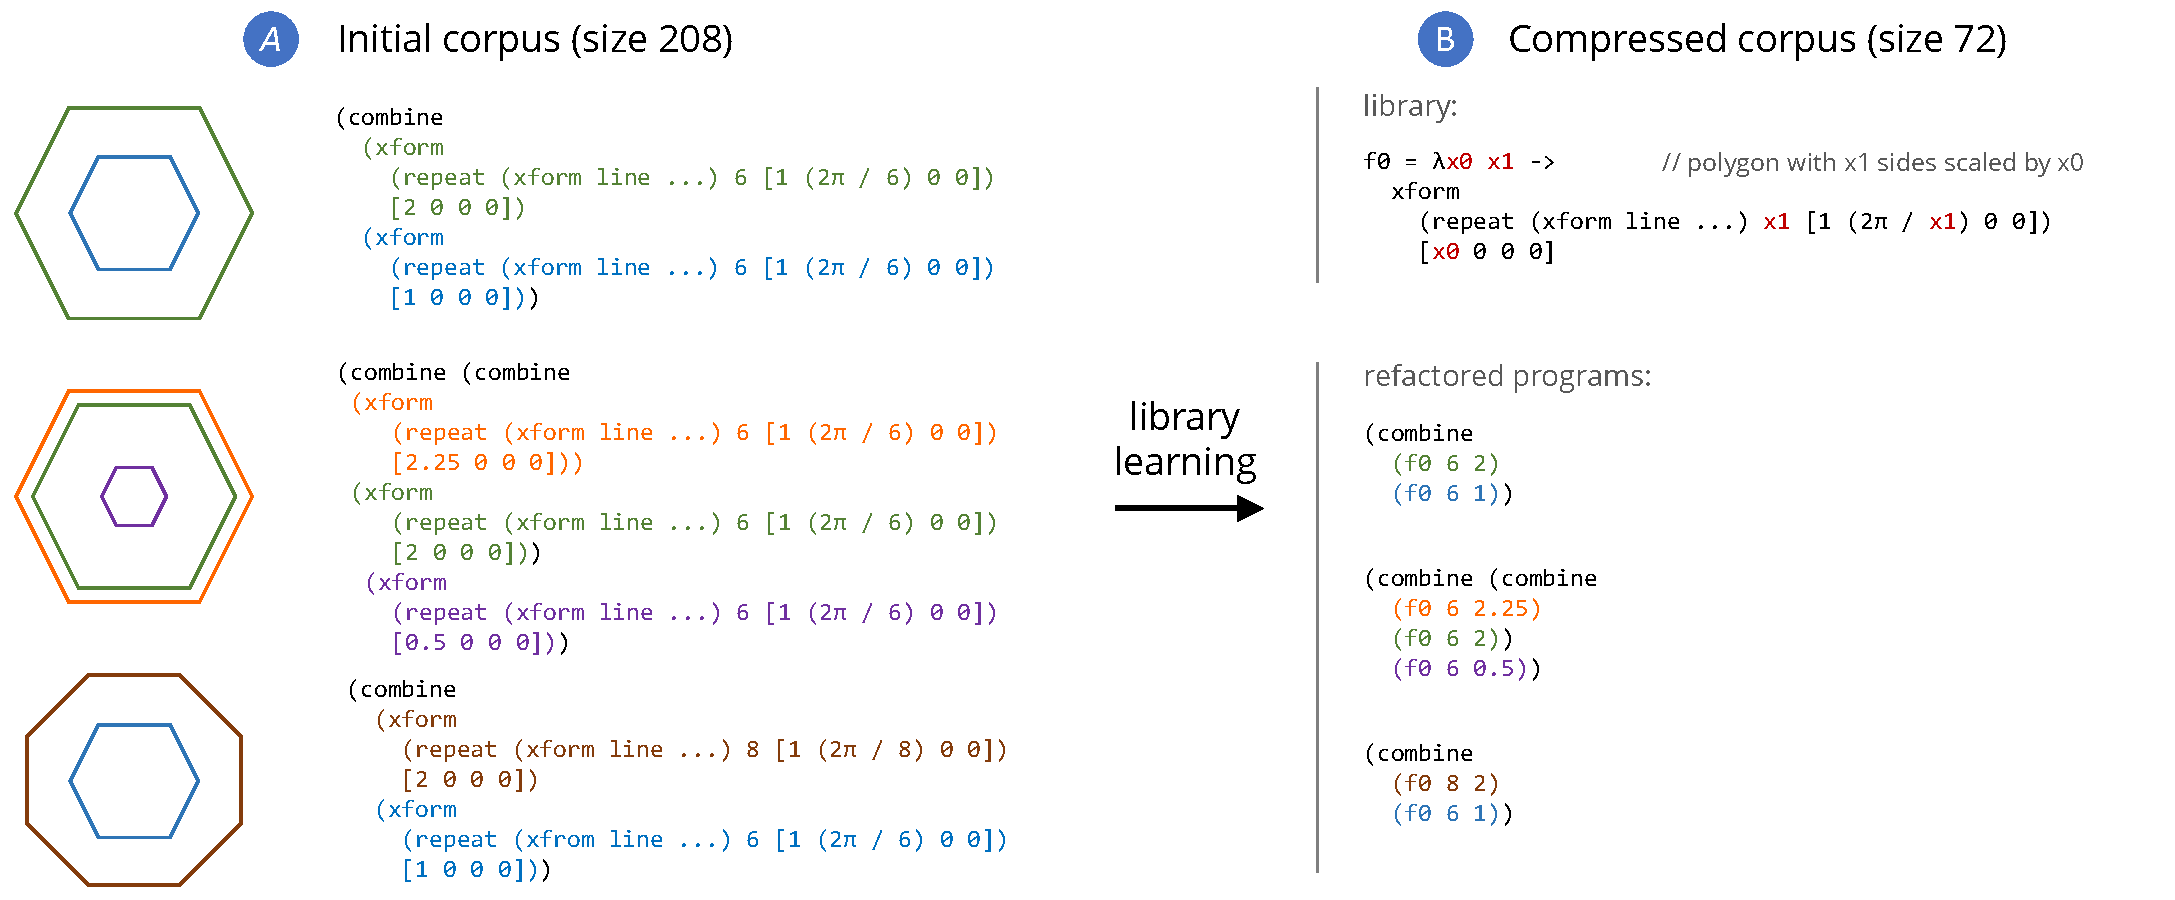
\includegraphics[width=\textwidth]{figures/polygons.pdf}
    \caption{Example of library learning.
             Initial corpus A contains three graphical programs from the ``nuts \& bolts'' dataset of \citet{cogsci-dataset}.
             Corpus B is the output of library learning with a single learned function for a scaled polygon,
             and the original programs refactored using this function.}\label{fig:polygons}
\end{figure}

\mypara{Limitations of Prior Work}
%
\dc's approach to library learning, called \emph{beta-inversion},
discovers library functions one at a time,
alternating between two stages:
\begin{enumerate*}[(1)]
    \item proposing candidate abstractions and
    \item selecting the optimal abstraction (the one that results in the best compression).
\end{enumerate*}
%
The first limitation of this approach is that the proposal stage is completely \emph{unguided}:
beta-inversion simply picks a random program fragment from the initial corpus
and replaces some of its arbitrarily chosen subterms with abstraction variables.
%
For example, to learn the function $f_0$ in \autoref{fig:polygons},
\dc would have to be lucky enough to pick, say, the orange subterm as a fragment,
\emph{and then also} decide to abstract over its subterms $6$ and $2.25$.
%
As a result, this approach does not scale beyond small corpora of short programs.

The second limitation beta-inversion
is that is can only extract purely \emph{syntactic} similarities between program fragments,
and hence it is \emph{not robust} to semantics-preserving variations in the input corpus.
%
For an example, let us take a closer look at \autoref{fig:polygons}.
%
Note that the terms for the two blue hexagons are of the form $\T{trans}\ (\T{repeat}\ \ldots)\ [1\ 0\ 0\ 0]$,
which amounts to scaling the underlying unit hexagon by 1!
%
This redundant transformation is crucial
for a syntactic library learning approach to generate the optimal abstraction $f_0$ from \autoref{fig:polygons}.
%
As shown in \autoref{fig:llmt},
eliminating this transformation
causes beta-inversion to learn a different function, $f_1$,
which abstracts over a unit (unscaled) polygon.
% Eliminating this transformation---%
% that is, simplifying both blue subterms to $\T{repeat}\ (\T{trans line}\ \ldots)\ 6\ [1\ (2\pi / 6)\ 0\ 0]$---%
% causes beta-inversion to instead learn the function:
% $$
% f_1 = \lambda x \bnd \T{repeat}\ (\T{trans line}\ \ldots)\ x\ [1\ (2\pi / x)\ 0\ 0]
% $$
% which abstracts over a unit (unscaled) polygon.
%
Although the simplified input corpus C from \autoref{fig:llmt}
is smaller than the original corpus A (196 AST nodes instead of 208),
its compressed version D is larger  (81 AST nodes instead of 72),
because the scaling transformation is now outside the abstraction and has to be repeated five times.

In this paper we propose \emph{library learning modulo (equational) theories} (LLMT)---%
a new library learning algorithm,
which addresses both of the above limitations.

\mypara{Scalability with Anti-Unification}
%
To make the proposal stage of library learning more efficient,
LLMT leverages two key observations:
\begin{enumerate*}[(1)]
    \item In order to be compressive, an abstraction must appear in the corpus at least twice;
    for example, there is no need to consider $\lambda x \bnd \T{trans}\ x\ [0.5\ 0\ 0\ 0]$ in our running example,
    because it can only be used in one place, thereby only increasing the size of the corpus.
    \item An abstraction cannot be optimal unless it captures all the common structure between the terms it abstracts;
    for example, there is no need to consider $\lambda x\ y to \T{repeat}\ (\T{trans line}\ \ldots)\ x\ y$ either,
    because everywhere this pattern occurs, $y$ actually has the shape $[1\ (2\pi / x)\ 0\ 0]$.
\end{enumerate*}
%
In other words, any viable candidate abstraction is a \emph{least general generalization} of some pair of subterms from the original corpus,
and can be computed via \emph{anti-unification} (AU)~\cite{plotkin1970lattice}.
%
For example, the abstraction $f_0$ can be computed by anti-unifying the green and the brown subterms of the corpus in \autoref{fig:polygons}.
%
The remaining challenge is to efficiently compute the set of anti-unifiers
between \emph{all} pairs of subterms in the corpus;
LLMT achieves this via a new bottom-up dynamic programming algorithm.

\begin{figure}
    \centering
    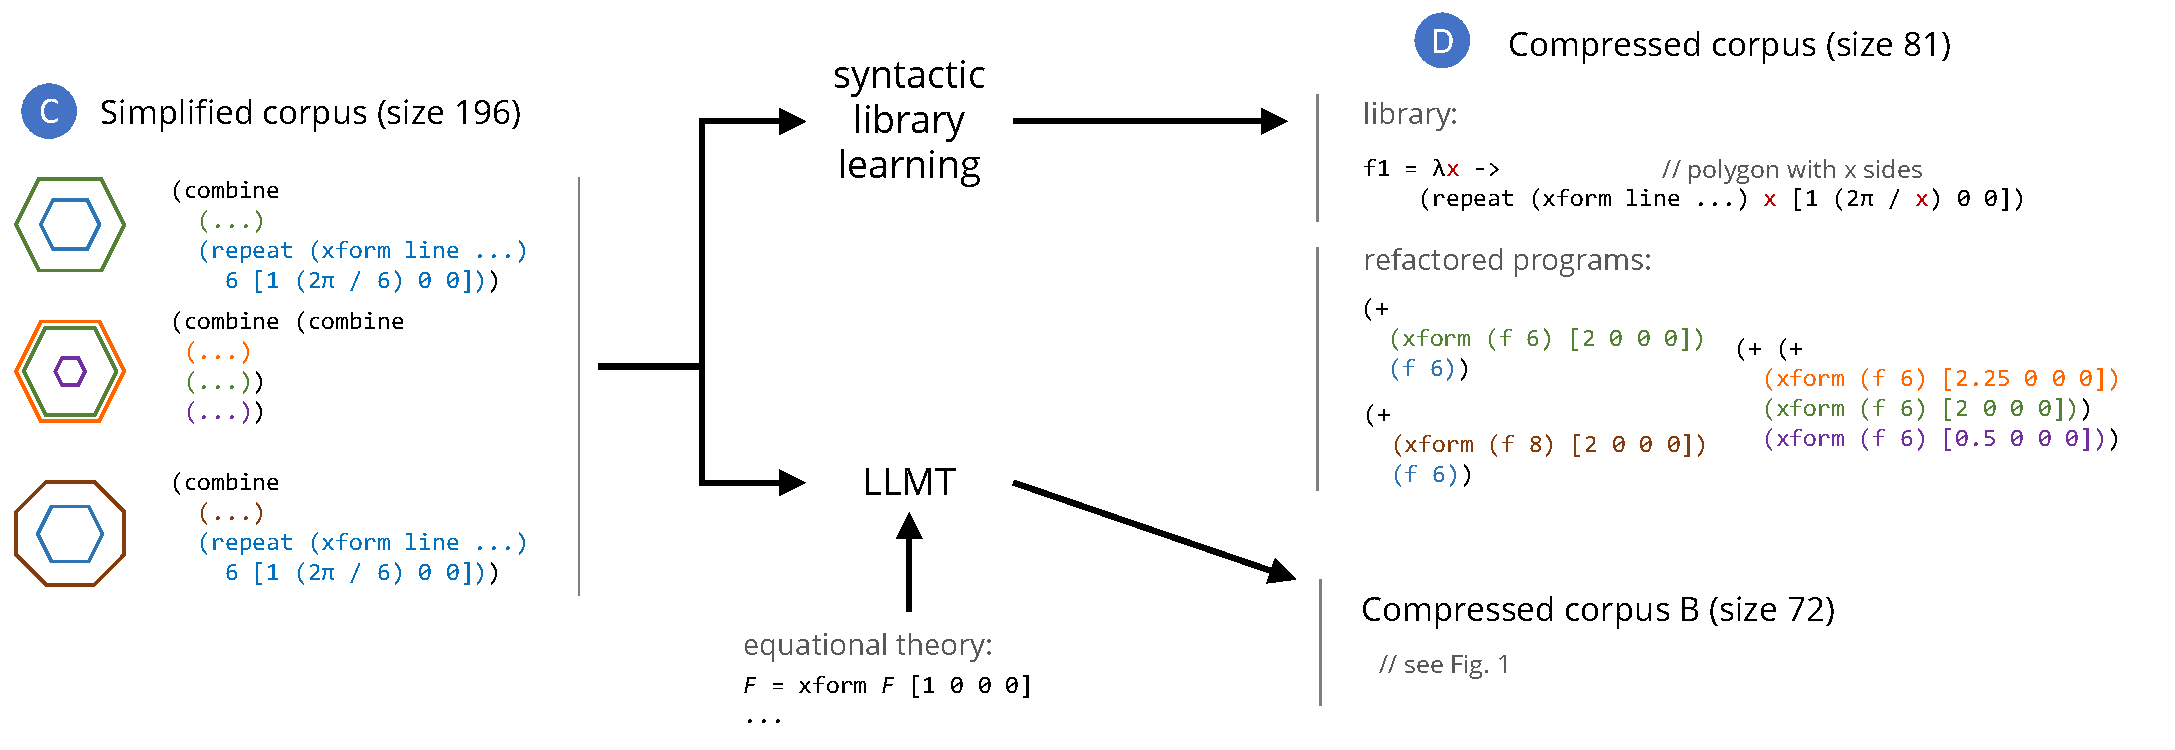
\includegraphics[width=\textwidth]{figures/polygons-simplified.pdf}
    \caption{Difference between syntactic library learning and LLMT.
             Here the initial corpus C is the simplified version of corpus A from \autoref{fig:polygons},
             with the redundant transformations on the blue subterms removed.
             With this modification, syntactic techniques would learn a suboptimal abstraction $f_1$,
             leading to corpus D,
             while LLMT still learns the optimal abstraction $f_0$.
     }\label{fig:llmt}
\end{figure}


\mypara{Robustness with E-Graphs}
%
To address the robustness issue,
LLMT additionally takes as input a domain-specific equational theory (expressed as a set of rewrite rules)
and uses it to find programs that are semantically equivalent to the original corpus,
but share the most syntactic structure.
%
For example, for the graphical DSL from our running example,
the equational theory might contain a rule that adds a unit transformation to any shape $s$:
$$
s  \Rightarrow  \T{trans}\ s\ [1\ 0\ 0\ 0]
$$
%
This rule can then be used to transform the two unit hexagons in corpus C from \autoref{fig:llmt}
into the form they have in the original corpus in \autoref{fig:polygons},
which enabled the discovery of the scaled polygon abstraction $f_0$
and using it to compress the corpus to size 72.

The main challenge with this approach is how do we represent and learn over the large space of programs
that are semantically equivalent to the original corpus.
%
To this end, LLMT relies on the \emph{e-graph} data structure
and the \emph{equality saturation} technique~\cite{tate2009equality,willsey2021egg}
to compute and represent the space of semantically equivalent programs.
%
To enable efficient library learning over this space,
we extend our AU-based algorithm for suggesting candidate abstractions to work over e-graphs.
%
We also propose a new algorithm for
  selecting the best subset of candidate abstractions,
  based on \emph{targeted common subexpression elimination}
  extraction for e-graphs.
\TODO{Do we need to talk about this? If we end up learning one at a time,
our selection algorithm is not that different from DC.}.
\TODO{ztatlock: I think it is ok to keep this?}





% Existing state-of-the-art: DreamCoder and Szalinski/smiley.
% - The former is a general system for lib learning... relies on guess and check, picks one function at a time. No semantic equiv, slow as fuck.
% - The latter are specific systems for doin lib learning in graphics domains.
%   But each has a kinda ad-hoc way of doing code compression. Doesn't work outside of their specific domains.
% - Also, all of these select one-at-a-time!

% To examine the existing solutions, we can break down the problem of lib learning into two parts.
% 1. Proposing candidate abstractions
% 2. Selecting the optimal set of abstractions

% We want general approach to proposal. It needs to handle both syntactic and semantic.
% And we want a better way to select optimal set.

\end{comment}
%%% Local Variables:
%%% mode: latex
%%% TeX-master: "main"
%%% End:

